\chapter{Analyse de Levee}
\label{chap:levee}

% introduction du projet Levee... composant, équipe, epfl

\gls{levee} est un projet mené dans le cadre du Dependable Systems Lab \cite{dslab} par les chercheurs Volodymyr Kuznetsov, Laszlo Szekeres, Mathias Payer, George Candea, R. Sekar et Dawn Song. Le but annoncé du projet est de sécuriser tout programme informatique contre la totalité des attaques de type \og control-flow hijack \fg via une erreur mémoire, du moment où celui-ci a été compilé grâce à \gls{clang} avec les options nécessaires.

Comme montré dans le chapitre précédent, il existe déjà plusieurs mécanismes (\gls{dep}, \gls{aslr}) permettant de réduire le risque de ce type d'attaque sans imposer au programme de coût supplémentaire en matière de performance. Cependant, il est aujourd'hui possible de les contourner, même au sein d'un environnement de production, grâce à des attaques évoluées telles que le \gls{rop}. D'autres mécanismes plus évolués (\gls{cfi}, SoftBound+CETS, CCured ou encore AddressSanitizer) permettent quant à eux d'améliorer très fortement la sécurité, mais ne permettent pas, soit de garantir une totale intégrité et reste à ce jour contournable, soit ils ne sont pas adoptés à grande échelle à cause de leurs effets beaucoup trop négatifs sur la performance du programme --- jusqu'à 116\% de coût en performance ---.

Le défi relevé par l'équipe de recherche a été de proposer un modèle de sécurité entraînant des coûts faibles en matière de performance tout en garantissant l'intégrité complète du flot de contrôle. \gls{levee} est le prototype d'implémentation de ce modèle et ce chapitre se concentre sur ses aspects théoriques, son implémentation au sein des outils de compilation \gls{llvm} et son rayon d'action.

\minitoc

\newpage

% -----------------------------------------------------------------------------
\section{Concepts théoriques}

Seules les attaques visant à dérouter le flot de contrôle de l'application sont prises en compte dans le modèle de sécurité. Les attaques du types \og data-only \fg, visant à modifier ou récupérer des informations qui ne font pas partie du flot de contrôle, n'entrent pas en considération.

Ils émettent l'hypothèse que l'attaquant a le contrôle total sur la mémoire du processus et que le chargement du programme ainsi que le binaire ne peuvent pas être altérés. De ce fait, les mécanismes de protection résultant de la compilation peuvent se mettre en place avant l'intervention de l'attaquant.

Les chercheurs du projet posent comme postulat de départ qu'il est suffisant de garantir l'intégrité des pointeurs pour rendre impossible la modification du flot de contrôle via l'exploitation d'erreurs mémoires. Dans le cas des langages de types \og memory-safe \fg, un objet en mémoire ne peut être accédé que depuis un pointeur prévu explicitement pour l'objet en question. Cela rend la modification du flot de contrôle impossible, mais entraîne une baisse de performances importante.

Afin de garder de bonnes performances tout en garantissant l'intégrité complète, un minimum d'instrumentation doit être délégué à l'exécution. Le code est alors en premier lieu analysé de manière statique à la compilation, puis des mécanismes de vérification sont ensuite délégués à l'exécution. Le concept de \og \gls{cpi} \fg \cite{CPIPaper} intervient alors, afin de déterminer quels pointeurs doivent être protégés, ce qui permet de réduire au minimum les accès à contrôler lors de l'exécution.


% -----------------------------------------------------------------------------
\section{\og Code-pointer integrity \fg (CPI)}

% Decrire pourquoi les pointeurs sensibles et pas sensibles. comment determiner si un pointeur est sensible

\subsection{Définition d'un \og code-pointer \fg}

Afin de formaliser les pointeurs de code \og code-pointers \fg, le papier propose la définition suivante :

\og On dit que l'indirection ou le déréférencement d'un pointeur est sûr si et seulement si l'adresse mémoire à laquelle il tente d'accéder est comprise au sein de l'\textit{objet mémoire} sur lequel le pointeur est \textit{basé}. Un \textit{objet mémoire} est une abstraction liée au langage définissant tout types de structures stockées en mémoire (variables globales, variables locales, structures, objets), de sous-structures (un champ d'une structure) ou encore des points de contrôle du flot (adresse de départ d'une fonction, adresse de retour). Ces \textit{objets mémoires} ont un cycle de vie défini, lorsqu'on libére la mémoire liée à un tableau et qu'on alloue un nouveau tableau avec la même adresse, un nouvel \textit{objet mémoire} est créé. \fg

Le papier formalise ensuite la définition de pointeur \textit{basé sur} un \textit{objet mémoire}. On dit qu'un pointeur est \textit{basé sur} sur un \textit{objet mémoire X} si et seulement si le pointeur est obtenu lors de l'exécution par (i) allocation de \textit{X} sur la pile, (ii) référencement explicite de l'adresse de \textit{X}, (iii) en référençant l'adresse d'un sous-objet \textit{y} de \textit{X} (accès au champ \textit{y} d'une structure \textit{X}), ou (iv) en effectuant une expression sur un pointeur (calculs arithmétiques, position au sein d'un tableau, copie de pointeur) impliquant l'adresse de l'\textit{objet mémoire X}. Cette définition est basée sur la définition des pointeurs \textit{basé sur} présente au sein de la norme \texttt{C99}.

\newpage

Si l'on part maintenant du principe que ces deux définitions sont strictement respectées pour tout pointeurs, peu importe les paramètres donnés à l'exécution du programme, alors on peut qualifier le-dit programme de \textit{memory-safe}. Dans ce cas il n'est plus possible de dérouter le flot de contrôle en exploitant une erreur basée sur la mémoire.

\subsection{Concept théorique}

Le mécanisme de \gls{cpi} est satisfait si toutes les indirections ou les déréférencements sur les pointeurs accédant ou déréférençant des pointeurs jugés \og sensibles \fg sont sûrs. La définition des pointeurs jugés sensibles est donc récursive. Les pointeurs de départ devant être protégés sont les pointeurs responsables de transférer le flot de contrôle de l'application. Cette notion de récursivité est donc dynamique, un pointeur de type \mintinline{c}{void*} doit être considéré comme sensible s'il pointe vers une fonction ou sur un autre pointeur jugé sensible, mais ne doit pas être considéré comme sensible s'il pointe vers un type \mintinline{c}{int}.

Les langages de programmation bénéficiant d'une mémoire supervisée satisfont le concept de \gls{cpi}. Cependant, ils ne différencient pas les pointeurs sensibles des autres, ce qui entraîne une forte baisse de performance par rapport aux langages de type \texttt{C/C++} (le papier mentionne une perte de $\geq2\times$ au sein des meilleures implémentations actuelles).

L'observation faite par l'équipe de chercheurs est la suivante: afin de garantir le flot de contrôle de l'application, seul l'accès aux pointeurs jugés sensibles doit être vérifié et ces pointeurs forment un ensemble de petite taille sur l'ensemble des pointeurs. Les pointeurs agissant sur les données peuvent se permettre de ne pas être contrôlés, ce qui augmente l'efficacité tout en maintenant un très haut taux de protection.

\subsection{Déterminer l'ensemble des pointeurs sensibles}
\label{subsection:detEnsemblePointeursSensible}

Afin de déterminer l'ensemble des pointeurs devant être considérés comme sensibles, une analyse statique est effectuée. Pour ce faire une heuristique simple est utilisée: \og un pointeur est jugé sensible si son type est sensible \fg. Les types marqués comme étant sensibles sont:

\begin{enumerate}
	\item les pointeurs de fonction
	\item les pointeurs pointant sur des pointeurs sensibles
	\item les pointeurs pointant sur des types composés (\mintinline{c}{array}, \mintinline{c}{struct}) qui contiennent un ou plusieurs pointeurs sensibles
	\item les pointeurs universels (\mintinline{c}{void*}, \mintinline{c}{char*})
  \item les pointeurs explicitements créés par le compilateur ou à l'exécution (adresse de retour, tables virtuelles en \texttt{C++} \cite{fonctionsVirtuelles}, \mintinline{c}{setjmp} \cite{setjmp})
\end{enumerate}

Cet ensemble de types peut être adapté, étendu, suivant les besoins du programme ou de la plateforme. Le papier mentionne en exemple la structure \mintinline{c}{ucred} utilisée dans le noyau FreeBSD, qui est marquée comme sensible car elle contient les UIDs des processus et d'autres informations.

En effectuant des tests, les chercheurs se sont rendu compte que l'analyse heuristique mettait en avant un ensemble de pointeurs correspondant en moyenne à $6.5\%$ de l'ensemble global. Ce chiffre met en avant l'impact sur l'efficacité qu'a cette approche.

Le coût en performance dépend directement de l'heuristique et de sa récursion. L'équipe mentionne elle-même que toutes les heuristiques donnant un ensemble approximatif cohérent peuvent être utilisées. Des améliorations peuvent encore être attendues sur ce point. Le second avantage majeur de cette approche réside dans le fait que l'on peut facilement imaginer de nouvelles heuristiques permettant de protéger d'autres ensembles de pointeurs, par exemple, pour protéger une partie des données au sein du programme.

\subsection{Zone de mémoire sûre}
\label{subsection:zoneMemoireSure}

Afin de garantir l'intégrité de l'ensemble des pointeurs sensibles, une zone mémoire appelée \og \textit{safe region} \fg est créée, voir la \autoref{fig:safeRegionLayout}. Cette région est isolée et ne peut être accédée que via des instructions fournies par \gls{cpi}. Cela permet de garantir l'intégrité des données et la propagation des métadonnées. Elle est ensuite constituée d'un \og \textit{safe pointer store} \fg, pour les pointeurs sensibles, et de \og \textit{safe stacks} \fg, pour une gestion plus spécifique liée à la pile d'exécution, voir la \autoref{section:safeStack}. Seule l'une des deux copies présente dans les deux régions est utilisée suivant le type du pointeur en question.

\begin{figure}[H]
	\centering
	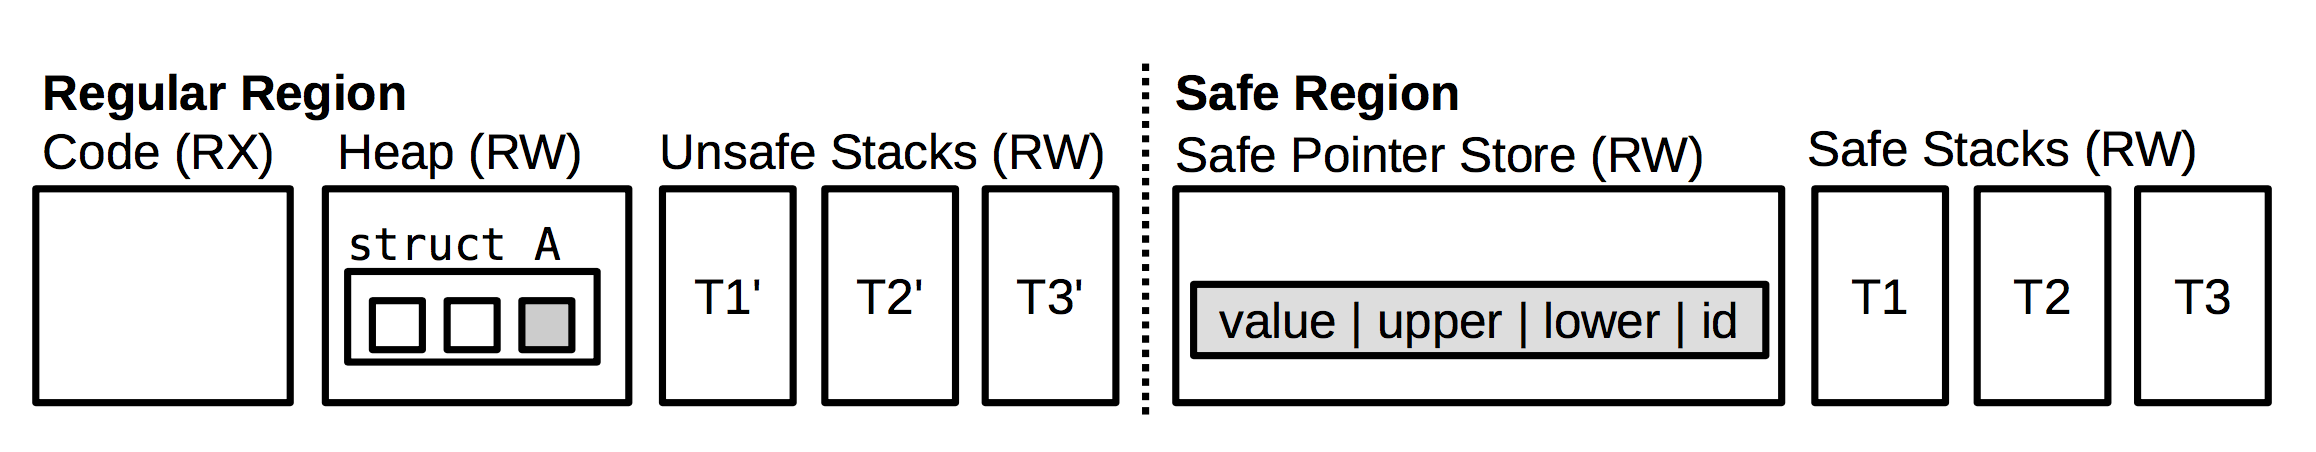
\includegraphics[width=1\columnwidth]{safeRegionLayout}
	\captionsource{Agencement de la mémoire avec CPI}
	{Agencement de la mémoire avec CPI, tiré du papier Code-Pointer Integrity}
	{\url{http://dslab.epfl.ch/pubs/cpi.pdf}}
	\label{fig:safeRegionLayout}
\end{figure}

Le \textit{safe pointer store} permet de stocker la valeur du pointeur et les métadonnées de l'\textit{objet mémoire} sur lequel le pointeur est \textit{basé}. Les métadonnées sont constituées de l'adresse de départ et de fin de l'objet au sein de la mémoire standard ainsi que d'un identifiant temporaire de l'objet en question. L'approche est similaire à celle utilisée au sein de SoftBounds+CETS \cite{SoftBound} à la différence prêt que \gls{cpi} stocke également la valeur du pointeur et n'applique pas de protection sur tout les pointeurs du programme.

\gls{cpi} garantit (i) que tous les pointeurs sensibles sont stockés dans la \og \textit{safe region} \fg, (ii) que la création et la modification lors de l'exécution de pointeurs sensibles soit propagée et (iii) que toutes les indirections ou les déréférences soient vérifiées grâce au métadonnées. Afin d'y parvenir, \gls{cpi}, lors de la phase de compilation, réécrit les instructions de création et d'accès de l'ensemble des pointeurs sensibles.


\subsection{Isolation de la zone mémoire sûre}
\label{subsection:isolationZoneMemoire}

Une fois les métadonnées et les \og \textit{safe stacks} \fg placées au sein de la région sûre, il faut pouvoir garantir leur intégrité. Pour ce faire cette région doit être isolée du reste de la mémoire et il ne doit pas être possible de la modifier sans passer par les instructions fournies par \gls{cpi}. Ce mécanisme de protection est directement dépendant de l'architecture pour laquelle le binaire est compilé. Dans tous les cas, la région sûre est placée dans le segment de \og memory mapping \fg avec un accès en lecture et écriture.

\subsubsection{Architecture 32~bits}

Dans le cas d'une architecture \texttt{x86-32}, la \og \textit{safe region} \fg est isolée grâce à l'utilisation des segments mémoires. Un segment mémoire n'étant pas utilisé au sein du programme est utilisé par \gls{cpi} afin de stocker l'adresse de base de la \og \textit{safe region} \fg. Les autres segments sont configurés afin de rendre l'accès à la région sûre impossible.

La preuve de sécurité sous cette architecture repose sur le fait qu'il n'est pas possible, lors de l'exécution, d'atteindre ou de modifier le segment qui contient la région de mémoire sûre.

\subsubsection{Architecture 64~bits}

Au sein d'une architecture \texttt{x86-64} la limitation des segments n'est plus présente, mais l'architecture met toujours à disposition deux registres de segments mémoire. \gls{cpi} utilise l'un des deux segments pour stocker l'adresse mémoire de base pour la \og \textit{safe region} \fg. Cette adresse de base est tirée aléatoirement lors du lancement de l'application, ce qui ressemble fortement à l'approche d'\gls{aslr} expliquée en \autoref{section:aslr}. Cependant, la différence mentionée dans le papier est qu'il n'existe aucun pointeur vers la \og \textit{safe region} \fg au sein de la région standard, ce qui fait qu'il n'est pas possible de remonter jusqu'à l'adresse de base. Les 48~bits d'adressage offrent donc une sécurité suffisante et rendent impraticable une attaque par recherche exhaustive.

La preuve de sécurité, sous architecture \texttt{x86-64}, est donc basée sur des informations cachées. Ils mentionnent le fait que leur modèle est \og leak-proof \fg \ --- c’est-à-dire qu'il ne laisse pas fuiter d'informations concernant la localisation de la région sûre ---, à la différence d'\gls{aslr}, grâce à l'absence de pointeur vers la \og \textit{safe region} \fg lors de l'exécution.


% -----------------------------------------------------------------------------
\section{\og Code-pointer separation \fg (CPS)}

Les chercheurs se sont rendus compte que dans le cas du \texttt{C++}, l'ensemble des pointeurs sensibles peut rapidement devenir trop important pour cause, par exemple, d'utilisation de fonctions virtuelles. Tous les pointeurs vers un objet contenant une fonction virtuelle deviennent alors sensibles, ce qui peut induire un coût de performance trop élevé. Pour palier à ce problème, le concept de \og \gls{cps} \fg a été mis en place. L'idée est de modifier quelque peu l'approche et de baisser les coûts en performance tout en garantissant le flot de contrôle.

Pour y arriver, l'heuristique utilisée pour définir l'ensemble des pointeurs lors de l'analyse statique ainsi que la définition d'un pointeur \textit{basé sur} sont modifiées. Seul les pointeurs pointant directement sur une destination du flot de contrôle sont protégés, laissant la récursion de côté. Contrairement à l'approche \gls{cpi}, il est possible de ne pas stocker de métadonnées dans la zone de mémoire sûre, en effet, en évitant par exemple les pointeurs sur des objets, chaque pointeur doit alors correspondre exactement à l'adresse de destination, les bornes ne sont plus nécessaires.

Les accès mémoires prennent alors, dans la majeur partie des cas (excepté pour les pointeurs de type universel), la même quantité de ressources qu'un programme sans \gls{cps}, à la différence que les pointeurs sensibles sont accédés et stockés dans la région sûre à la place de leur emplacement original.

\newpage

Les chiffres avancés au niveau des gains en performance de \gls{cps} sont de l'ordre de $4.3\times$ plus rapide que \gls{cpi}. Le coût mesuré passe alors de $8.4\%$ à $1.9\%$. Évidemment ces chiffres dépendent de l'ensemble des pointeurs à protéger et donc dirrectement de l'architecture dudit programme.


% -----------------------------------------------------------------------------
\section{\og Safe Stack \fg}
\label{section:safeStack}

Le composant \og \gls{safeStack} \fg est un équivalant, mais potentiellement plus complet, aux \og \gls{stackCookies} \fg. Son but est de protéger les variables sensibles stockées sur la pile d'exécution. Pour ce faire, à la manière dont fonctionne \gls{cpi}, \og \gls{safeStack} \fg sépare les variables dans deux régions mémoires différentes. Cependant, dans le cas de \og \gls{safeStack} \fg, l'approche est différentes. Seules sont déplacées les variables dont l'allocation ou les accès sont considérés comme non-sécurisés. Les allocations et les accès à ces variables sont ensuite remplacés lors de la phase de compilation par \og \gls{safeStack} \fg afin de les initialiser dans une zone mémoire non protégée. Cette zone mémoire est initialisée au lancement de l'application, au sein du segment de \og memory mapping \fg.

Comme montré sur la \ref{fig:safeRegionLayout}, la zone mémoire sûre, ou région sûre, est constituée d'une ou plusieurs \og safe stacks \fg. Chaque \og safe stack \fg appartient à un \texttt{thread}, celui-ci contient un pointeur vers la pile standard et un pointeur vers la pile sûre. Le registre \mintinline{c}{%esp} sur l'architecture \texttt{x86-32} pointe vers la \og \gls{safeStack} \fg --- \mintinline{c}{%rsp} sur \texttt{x86-64} ---, tandis qu'une variable locale au \texttt{thread} pointe vers la \og unsafe stack \fg, présente dans le segment de \og memory mapping \fg.

\subsection{Analyse à la compilation}
\label{subsection:analyseCompilation}

Il est nécessaire de passer par un phase d'analyse afin de determiner, comme pour \gls{cpi}, quelles variables déplacer.
La fonction \mintinline{c}{IsSafeStackAlloca()} détermine quels types de variables peuvent être accédés de manière non-sécurisée. Une variable est déclarée non-sécurisée si l'un des critères est retenu:

\begin{enumerate}
	\item un pointeur vers la variable est stocké quelque part en mémoire;
	\item un élément appartenant à un tableau est accédé par un index non-constant (une autre variable);
	\item un tableau dynamique est accédé (via une variable ou un index constant);
	\item un pointeur vers la variable est donnée en arguement à une fonction.
\end{enumerate}

\subsection{Support à l'exécution}

Afin d'initialiser et gérer les allocations mémoires de la zone non-sécurisée, une bibliothèque est fournie à l'exécution. Plus de détails sont donnés dans la \autoref{subsection:architectureSafeStack}.

% -----------------------------------------------------------------------------
\section{Implémentation au sein de LLVM}

% version de LLVM, depuis quand, sous quel nom, documentation
%
% structure de LLVM front-end, l'optimizer, et le back-end, son fonctionnement, origine

La première implémentation de \gls{levee} a été portée au sein de la version 3.3 de \gls{llvm} (juin 2013). Pour ce prototype, l'équipe de \gls{levee} a dû modifier quelque peu l'infrastructure, des modifications ont été faites sur les bibliothèques de \gls{llvm} ainsi que dans \gls{clang}. Depuis la version 3.8, en mars 2016, \og \gls{safeStack} \fg est disponible au sein de \gls{llvm} et \gls{clang}, cette intégration a été faite par un employé de Google, Peter Collingbourne. Actuellement, en mai 2017, dans la version 4.0 de \gls{llvm}, les prototypes de \gls{cpi} et \gls{cps} ne sont toujours pas présents et aucune date d'intégration n'a été annoncée.

\subsection{Historique de LLVM}

Le projet débute dans le début des années 2000, par ce qui est au début un travail de recherche universitaire de Chris Lattner \cite{ChrisLattner}. À cette époque, il est courant de voir pour les compilateurs une implémentation monolitique, par exemple GCC pour la famille des langages \texttt{C}. Au sein de ces implémentations, Lattner remarque qu'il est également difficile de réutiliser du code pour servir différents intérêts, utiliser l'analyseur --- \og parser \fg --- de GCC pour effectuer une analyse statique n'est pas possible et les parties de code en commun sont relativement petites.

Lattner propose alors une collection, open source, souple et réutilisable, de technologies permettant de développer des \og frontends \fg et \og backends \fg de compilateur. Le design le plus populaire utilisé par les compilateurs est constitué de trois phases, (i) le \og frontend \fg, responsable d'analyser le code et de générer une représentation abstraite --- appelée \og \gls{ast} \fg \ --- (ii) l'\og optimizer \fg, améliore cette représentation (suppression des redondances, simplification des opérations mathématiques, etc.), puis (iii) le \og backend \fg, transcrit la représentation intermédiaire en code machine suivant la plateforme ciblée.

\begin{figure}[H]
	\centering
	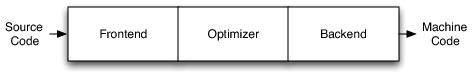
\includegraphics[width=0.7\columnwidth]{SimpleCompiler}
	\captionsource{Composants majeurs d'un compilateur en trois phases}
	{Composants majeurs d'un compilateur en trois phases}
	{\url{http://www.aosabook.org/en/llvm.html}}
	\label{fig:SimpleCompiler}
\end{figure}

Il y a plusieurs avantages majeurs à cette approche, premièrement lorsque l'on souhaite supporter un nouveau langage, seul le \og frontend \fg doit être écrit. De la même manière, si l'on souhaite rajouter une plateforme, les \og frontend \fg existant peuvent facilement en profiter. Deuxièmement, au niveau des projets open source, il est très avantageux d'avoir, au sein du même projet, différents langages ciblés, car cela accroît la communauté potentielle et donc le nombre de contributeurs. En finalité, le fait qu'il n'est pas nécessaire d'avoir les mêmes compétences pour écrire un \og frontend \fg, un \og optimizer \fg ou un \og backend \fg aide à trouver des contributeurs, un projet open source veut réduire au maximum le pas à franchir pour contribuer.

\begin{figure}[H]
	\centering
	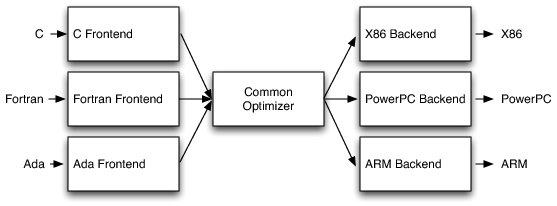
\includegraphics[width=0.6\columnwidth]{RetargetableCompiler}
	\captionsource{Modularité d'une structure en trois phases}
	{Modularité d'une structure en trois phases}
	{\url{http://www.aosabook.org/en/llvm.html}}
	\label{fig:RetargetableCompiler}
\end{figure}

Dans un premier temps, \gls{llvm} est l'acronyme de \og low level virtual machine \fg, mais rapidement le projet se développe et le nom \gls{llvm} devient une marque rassemblant sous son nom différents projets tel que \gls{llvmIR}, \gls{lldb}, LLD ou encore LLVM \texttt{C++ Standard Library}, une implémentation de la bibliothèque standard \texttt{C++11} et \texttt{C++14}.

\subsection{Structure de LLVM}

\gls{llvm} reprend le design des trois phases et l'implémente en plusieurs parties. Parmi ces parties, le langage intermédiaire joue un très grand rôle. C'est lui qui donne le plus de sens à l'architecture choisie et qui rend si puissant \gls{llvm}.

\begin{figure}[H]
	\centering
	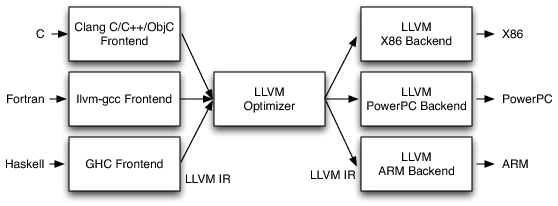
\includegraphics[width=0.7\columnwidth]{LLVMCompiler1}
	\captionsource{Vue d'ensemble des composants de LLVM}
	{Vue d'ensemble des composants de LLVM}
	{\url{http://www.aosabook.org/en/llvm.html}}
	\label{fig:LLVMCompiler1}
\end{figure}

\subsubsection{Représentation intermédiaire}

\gls{llvmIR} est un langage en soit, normé et bien défini, fortement typé, ayant pour seul but de répondre aux besoins de l'optimisation. Sa définition en fait un langage permettant d'être très fortement modifié et restructuré lors de la phase en question.

\begin{listing}
	\bashfile{02-main/listings/sample.ll}
	\caption{Example de code \gls{llvmIR}, source : \url{http://www.aosabook.org/en/llvm.html}}
	\label{lst:sampleLLIR}
\end{listing}

La représentation \autoref{lst:sampleLLIRC} est le résultat du code \texttt{C} en \autoref{lst:sampleLLIR}. Le défi réside dans la propagation des informations, lorsque l'on transforme du code \texttt{C} en une quelconque autre représentation, certaines informations peuvent être perdues. Lorsque l'équipe de \gls{levee} a commencé à travailler sur le projet, ils se sont rendu compte que certaines informations étaient perdues lors de la transformation en \gls{llvmIR} et ont dû compléter les métadonnées émises par \gls{clang}.

\begin{listing}
	\cfile{02-main/listings/sample.c}
	\caption{Code source \texttt{C} de l'exemple de représentation intermédiaire, source : \url{http://www.aosabook.org/en/llvm.html}}
	\label{lst:sampleLLIRC}
\end{listing}

Le langage intermédiaire \gls{llvmIR} est constitué d'instructions ressemblant fortement au langage machine, mais à quelques différences. De manière non-exhaustive, (i) les conventions d'appel de \texttt{ret} ou \texttt{call} sont abstraites --- c'est au \og backend \fg de se soucier de ce genre de conventions ---, (ii) un nombre infini de variables commençant par \texttt{\%} est à disposition et (iii) celles-ci sont typées grâce à un système simple: \texttt{i32} pour un entier de 32~bits, \texttt{i32**} pour un pointeur de pointeur sur un entier de 32~bits, et cetera.

\gls{llvmIR} peut être stocké et manipulé sous trois forme différentes: (i) la forme textuelle, comme montrée en \autoref{lst:sampleLLIR}, (ii) sous forme de données structurées en mémoire --- forme utilisée par les optimiseurs --- et (iii) sous une forme de \og bitcode \fg, sauvegardée sur le disque, permettant une gestion plus efficace et plus dense de l'information. Des outils de conversion du \og bitcode \fg (\texttt{.bc}) au format textuel (\texttt{.ll}) et vice versa sont présents dans la suite \gls{llvm}.

\subsubsection{LLVM \og frontends \fg}

\gls{llvmIR} est la seule interface au sein de \gls{llvm}, ce qui signifie que le seul pré-requis pour écrire un \og frontend \fg \gls{llvm} est de connaître son fonctionnement. Du fait que ce langage soit un langage textuel, il suffit au \og frontend \fg d'écrire le résultat dans un fichier texte et une simple commande tel que les \og Unix pipes \fg permettent de profiter de tout la suite de l'infrastructure.

\subsubsection{LLVM \og optimizers \fg}

Le fonctionnement d'un \og optimizer \fg est plutôt simple: il prend en entrée le code sous forme de la représentation intermédiaire et produit du code, toujours sous la forme \gls{llvmIR}, normalement plus efficace. Les \og optimizers \fg sont organisés sous forme de pipeline, chaque \og optimizer \fg représente une \og pass \fg dans celui-ci. Suivant le niveau d'optimisation souhaité lors de la compilation, par exemple \texttt{-O3}, le plus haut niveau, le nombre de \og pass \fg fluctue.

Chaque \og pass \fg au sein de \gls{llvm} est écrite en \texttt{C++} et dérive --- indirectement --- de la classe \texttt{Pass}. Les \og pass \fg doivent être les plus indépendantes possible les unes des autres, leur architecture permet d'inclure seulement les \og pass \fg utilisées lors de la compilation.

\begin{figure}[H]
	\centering
	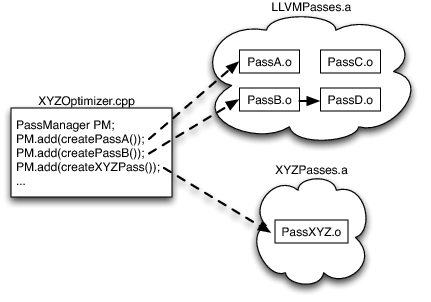
\includegraphics[width=0.6\columnwidth]{PassLinkage}
	\captionsource{Exemple de construction d'un optimiseur LLVM}
	{Exemple de construction d'un optimiseur LLVM}
	{\url{http://www.aosabook.org/en/llvm.html}}
	\label{fig:PassLinkage}
\end{figure}

L'interface, très claire, des \og pass \fg permet une très grande modularité ainsi qu'une certaine puissance et cela laisse la possibilité d'implémenter n'importe quelle fonctionnalité au sein de \gls{llvm}.

\subsubsection{LLVM \og backends \fg}

La transcription entre le langage intermédiaire et le code machine est géré par le composant \og LLVM code generator \fg. Il est nécessaire de produire le code le plus spécifique et le plus optimisé sur chaque plateforme, de ce fait il est préférable que chaque \og backend \fg produise un code machine unique. Cependant, il est aussi intéressant de pouvoir partager une partie de la logique parmi --- par exemple l'allocation des variables \texttt{\%} au sein des registres ---. Pour ce faire, le système de \og pass \fg est également appliqué lors de la génération du code machine.

\gls{llvm} met à disposition une liste de \og pass \fg présentes par défaut, répondant à des problématiques récurentes, ainsi l'auteur de la plateforme ciblée peut choisir de redéfinir certaine \og pass \fg, de les enlever ou d'en rajouter.

Cette approche amène alors le défi de fournir des \og pass \fg génériques, mais spécifiques à chaque plateforme. \gls{llvm} répond à ce défi grâce à un langage spécifique, les \og LLVM target description files \fg (\texttt{.td}), permettant de fournir, pour chaque plateforme, la description de celle-ci pour la \og pass \fg en question.

\begin{figure}[H]
	\centering
	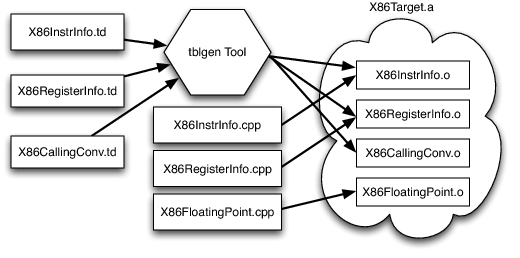
\includegraphics[width=0.6\columnwidth]{X86Target}
	\captionsource{Simplification du processus de définition spécifique à la plateforme \texttt{x86}}
	{Simplification du processus de définition spécifique à la plateforme \texttt{x86}}
	{\url{http://www.aosabook.org/en/llvm.html}}
	\label{fig:X86Target}
\end{figure}

\vfill

\begin{listing}
	\begin{minted}[breaklines=true,fontsize=\scriptsize]{text}
def GR32 : RegisterClass<[i32], 32,
  [EAX, ECX, EDX, ESI, EDI, EBX, EBP, ESP,
   R8D, R9D, R10D, R11D, R14D, R15D, R12D, R13D]> { … }
	\end{minted}
	\caption{Description des registres disponibles pour le \og backend \fg \texttt{x86}}
	\label{lst:x86RegisterTd}
\end{listing}

Le \autoref{lst:x86RegisterTd} est un exemple de \texttt{.td} décrivant les registres à disposition pour la plateforme \texttt{x86}. Différentes informations sont présentes, par exemple le fait que les registres sont en 32~bits, de préférence alignés, etc. D'autres informations tel que l'ordre d'utilisation préféré sont décrites dans ces fichiers.

\subsection{Implémentation de CPI}

L'implémentation de \gls{cpi} commme \gls{levee} le propose au sein de la version 3.3 de \gls{llvm} est composée de deux \og pass \fg. La première permettant d'identifier les pointeurs sensibles selon le design expliqué en \autoref{subsection:detEnsemblePointeursSensible} et la deuxième permettant de mettre en place la séparation des pointeurs et d'assurer leur intégrité commen expliqué en \autoref{subsection:zoneMemoireSure} et en \autoref{subsection:isolationZoneMemoire}.

Comme mentioné précédement, il se peut que de l'information soit perdue lors de la transformation du code source en \gls{llvmIR}. Dans le cas de cette implémentation, le cas de figure c'est imposé. \gls{clang} ne conservait pas le type original des pointeurs étant transformé en \mintinline{c}{void*} quand ceux-ci sont passés à la fonction \mintinline{c}{memset} par exemple. Ou encore que \gls{llvmIR} ne faisait pas la différence entre un pointeur de type \mintinline{c}{void*} et \mintinline{c}{char*} --- les deux étant représenté par un \texttt{i8*} ---, ce qui est une information utile dans le cas de \gls{cpi}. L'équipe a donc dû améliorer \gls{clang} afin de préserver ces informations lors du passage du \texttt{C/C++} au \gls{llvmIR} entant que \og LLVM metadata \fg.

La seconde \og pass \fg permettant de mettre en place l'instrumentation rajoute, dans la plupart des cas, des appels aux fonctions tels que \mintinline{c}{cpi_ptr_store()} ou encore \mintinline{c}{cpi_memcopy()}. Ces fonctions sont implémentées au sein du \og \texttt{compiler-rt} \fg et sont compilées entant que \og LLVM bitcode \fg puis liées aux objets compilés par \gls{clang}.

\subsection{Architecture de \og safe stack \fg}
\label{subsection:architectureSafeStack}

L'implémentation de \og \gls{safeStack} \fg, dans la version 4.0 de \gls{llvm}, est découpée en deux parties: (i) une \og pass \fg d'analyse et d'optimisation et (ii) l'implémentation de la bibliothèque d'exécution.

\subsubsection{Anaylse et optimisation}

Une seule \og pass \fg au sein de l'\og optimizer \fg est résponsable d'appliquer \og \gls{safeStack} \fg et est présente sous le nom de \texttt{SafeStackLegacyPass}.

La classe implémente plusieurs méthodes dont (i) une méthode permettant de vérifier une allocation donnée, (ii) une méthode permettant de déplacer les variables non-sécurisée statiques, (iii) une méthode permettant de déplacer les variables non-sécurisée dynamiques ou encore (iv) une méthode permettant d'appliquer \og \gls{safeStack} \fg sur une fonction donnée.

\newpage

\begin{listing}
	\begin{minted}[breaklines=true,fontsize=\scriptsize]{c}
/// The SafeStack pass splits the stack of each function into the safe
/// stack, which is only accessed through memory safe dereferences (as
/// determined statically), and the unsafe stack, which contains all
/// local variables that are accessed in ways that we can't prove to
/// be safe.
class SafeStackLegacyPass : public FunctionPass {

  /// \brief Allocate space for all static allocas in \p StaticAllocas,
  /// replace allocas with pointers into the unsafe stack and generate code to
  /// restore the stack pointer before all return instructions in \p Returns.
  ///
  /// \returns A pointer to the top of the unsafe stack after all unsafe static
  /// allocas are allocated.
  Value *moveStaticAllocasToUnsafeStack(IRBuilder<> &IRB, Function &F,
                                        ArrayRef<AllocaInst *> StaticAllocas,
                                        ArrayRef<Argument *> ByValArguments,
                                        ArrayRef<ReturnInst *> Returns,
                                        Instruction *BasePointer,
                                        AllocaInst *StackGuardSlot);

  /// \brief Replace all allocas in \p DynamicAllocas with code to allocate
  /// space dynamically on the unsafe stack and store the dynamic unsafe stack
  /// top to \p DynamicTop if non-null.
  void moveDynamicAllocasToUnsafeStack(Function &F, Value *UnsafeStackPtr,
                                       AllocaInst *DynamicTop,
                                       ArrayRef<AllocaInst *> DynamicAllocas);

  bool IsSafeStackAlloca(const Value *AllocaPtr, uint64_t AllocaSize);

  bool IsMemIntrinsicSafe(const MemIntrinsic *MI, const Use &U,
                          const Value *AllocaPtr, uint64_t AllocaSize);

  bool IsAccessSafe(Value *Addr, uint64_t Size, const Value *AllocaPtr,
                    uint64_t AllocaSize);

public:
	bool runOnFunction(Function &F) override;
}
	\end{minted}
	\caption{Déclaration partielle de la classe \og \gls{safeStack} \fg montrant certaines des méthodes mentionnées}
	\label{lst:SafeStackLegacyPassClass}
\end{listing}

La méthode \mintinline{c}{runOnFunction()} permet de séparer la pile d'exécution, si besoin est, de la fonction passée en paramètre. C'est le point de départ de l'analyse et de l'instrumentation de \og \gls{safeStack} \fg. Cette méthode fait appel à \mintinline{c}{IsSafeStackAlloca()}, voir \autoref{lst:IsSafeStackAllocaHeader}, permettant de determiner si une allocation doit être déplacée ou non, selon les explications en \autoref{subsection:analyseCompilation}.

\begin{listing}
	\begin{minted}[breaklines=true,fontsize=\scriptsize]{c}
/// Check whether a given allocation must be put on the safe
/// stack or not. The function analyzes all uses of AI and checks whether it is
/// only accessed in a memory safe way (as decided statically).
bool SafeStack::IsSafeStackAlloca(const Value *AllocaPtr, uint64_t AllocaSize);
	\end{minted}
	\caption{Signature de la méthode permettant de déterminer si une allocation est sûre}
	\label{lst:IsSafeStackAllocaHeader}
\end{listing}

La méthode \mintinline{c}{moveStaticAllocasToUnsafeStack()}, voir \autoref{lst:moveAllocasToUnsafeStack}, ainsi que la méthode  \mintinline{c}{moveDynamicAllocasToUnsafeStack()} permettent de générer et remplacer le code nécessaire afin de modifier les allocations marquées par la méthode \mintinline{c}{IsSafeStackAlloca()}. Lors de l'appel à la méthode \mintinline{c}{runOnFunction()} les allocations des variables statiques sont dabord modifiées, puis un pointeur vers le haut de la pile non-sécurisée est récuperé avant de modifier les allocations dynamiques, partant dudit pointeur.

\begin{listing}
	\begin{minted}[breaklines=true,fontsize=\scriptsize]{c}
/// \brief Allocate space for all static allocas in \p StaticAllocas,
/// replace allocas with pointers into the unsafe stack and generate code to
/// restore the stack pointer before all return instructions in \p Returns.
///
/// \returns A pointer to the top of the unsafe stack after all unsafe static
/// allocas are allocated.
Value *moveStaticAllocasToUnsafeStack(IRBuilder<> &IRB, Function &F,
                                      ArrayRef<AllocaInst *> StaticAllocas,
                                      ArrayRef<Argument *> ByValArguments,
                                      ArrayRef<ReturnInst *> Returns,
                                      Instruction *BasePointer,
                                      AllocaInst *StackGuardSlot);

/// \brief Replace all allocas in \p DynamicAllocas with code to allocate
/// space dynamically on the unsafe stack and store the dynamic unsafe stack
/// top to \p DynamicTop if non-null.
void moveDynamicAllocasToUnsafeStack(Function &F, Value *UnsafeStackPtr,
                                     AllocaInst *DynamicTop,
                                     ArrayRef<AllocaInst *> DynamicAllocas);
	\end{minted}
	\caption{Signatures des méthodes permettant de déplacer les allocations dans la zone non-sécurisée}
	\label{lst:moveAllocasToUnsafeStack}
\end{listing}

Afin de lire et comprendre toute l'implémentation de \og \gls{safeStack} \fg dans la version 4.0, vous trouverez \og \gls{safeStack} \fg sur le dépôt miroire de \gls{llvm} disponible \href{https://github.com/llvm-mirror/llvm/blob/release_40/lib/CodeGen/SafeStack.cpp}{ici}. Le commit ajoutant \og \gls{safeStack} \fg à \gls{llvm} est disponible \href{https://github.com/llvm-mirror/llvm/commit/7ffec838a2b72e6841d9fb993b5fe6a45f3b2a90#diff-0ae4221c82094c2703f2511b921530e0}{ici}.

\subsubsection{Bibliothèque d'exécution}

% implemented as a compiler-rt library that is automatically linked in when the program is compiled with SafeStack

Comme pour \gls{cpi}, \og \gls{safeStack} \fg est dotée d'une bibliothèque permettant de géréer son initialisation. On retrouve dans cette bilbiothèque les fonctions s'occupant d'intercépter les événements des \texttt{threads} afin d'initialiser et libérer les piles d'exécution non-sécurisées, ainsi que les fonctions de gestion de la pile, voir \autoref{lst:safeStackRuntime}. L'implémentation complète est disponible, dans sa version 4.0, \href{https://github.com/llvm-mirror/compiler-rt/blob/release_40/lib/safestack/safestack.cc}{ici}.


% -----------------------------------------------------------------------------
\section{Rayon d'action}

% qu'est qu'il est sensé proteger par rapport au chapitre historique

La combinaison \gls{cpi} et \og \gls{safeStack} \fg permet effectivement de couvrire tout les attaques contre le flot de contôle se basant sur une erreur provenant de la gestion de la mémoire. La protection \og \gls{safeStack} \fg seule, tel qu'implémentée au sein de \gls{llvm} actuellement, permet de se prémunir contre les dépassements de tampon ayant lieu uniquement sur la pile d'exécution. \og Safe stack \fg ne couvre donc qu'une partie des attaques connues au jour d'aujourd'hui.

\subsection{\og Safe stack \fg ou canaris}

\og Safe stack \fg est désigné comme équivalant, voir en remplacement des canaris. La question se pose alors, quels sont les avantages de \og \gls{safeStack} \fg sur les canaris ? La mise en pratique d'une attaque, voir \autoref{chap:attaque}, a montré que seul certains cas particuliers supplémentaires sont couvert par \og \gls{safeStack} \fg. L'implémentation n'introduit pas de coût en performance significatif et est au même niveau des \og \gls{stackCookies} \fg, les quelques pourcent de couverture supplémentaire sont donc bienvenus.
